\chapter{Použitý model}\label{model}

Jak vypadá.

Jak souvisí s MIL, jak se liší.

Hledání funkce \( \phi \) - neuronové sítě. Použité vrstvy. ADAM (možná i shrnutí jiných metod - SGD, ADAMax...)

\null

Jelikož úloha představená v kapitole \ref{problem} je úlohou v níž je adresa URL rozdělena na části a ty jsou posléze rozděleny na podčásti, je na model použitý k aproximaci klasifikační funkce kladen požadavek, aby reflektoval tuto hierarchickou strukturu vstupních dat. Použitý model využívá přístupu pomocí multi-instančního učení \footnote{resp. jeho speciální varianty, popsané v kapitole \ref{MIL-modification}.}, popsaného v kapitole \ref{MIL}, aplikovaného dvakrát na sebe sama. Tím je umožněno modelovat nejprve tři vybrané části adresy URL (doménu, cestu a dotaz) z jejich podčástí, a posléze z těchto tří částí modelovat samotnou adresu URL.

\section{Reprezentace adresy URL pomocí tašek vektorů}

V kapitole \ref{problem} byla definována abeceda všech znaků přípustných v adrese URL \( \Sigma \) jako abeceda malých a velkých písmen anglické abecedy, čísel a znaků \$ - \_ . + ! * ' ( ) , \% ; / ? : @ \& = (srov. \cite{berners-lee_uniform_1994}). Každá adresa URL, každá její část i podčást je slovem v abecedě \( \Sigma \). Aby však bylo možné s těmito objekty dále pracovat, je zapotřebí je převést na vektory. Toho je dosáhnuto pomocí nějaké funkce \( \psi : \Sigma^* \to \BPfield R^n \) kde symbolem \( \Sigma^* \) je označována množina všech slov nad abecedou \( \Sigma \). Tím je definován prostor vstupních objektů, dále nazývaných \BPname{vektory příznaků} (\BPenname{feature vectors}), jako
\[ \BPspace X_1 = \psi \left( \Sigma^* \right) \subset \BPfield R^n \]
Tento prostor obsahuje všechny vektory příznaků odpovídající podčástem adresy URL. Prostor \( \BPspace B_1 \subset \BPspace P^M \left( \BPspace X_1 \right) \) je tedy konstruován tak, že každá taška v \( \BPspace B_1 \) odpovídá vektorům příznaků podčástí jedné části jedné adresy URL. Za použití paradigmatu vloženého prostoru, popsaného v kapitole \ref{embedded-space-paradigm} lze najít nějakou vkládající funkci
\[ \phi_1 : \BPspace B_1 \to \BPspace X_2 \]
kde \( \BPspace X_2 \) je opět nějaký vstupní prostor, který může, ale nemusí být totožný s \( \BPspace X_1 \). Nad tímto prostorem je konstruován prostor tašek \( \BPspace B_2 \subset \BPspace P^M \left( \BPspace X_2 \right) \) tak, že každá taška v prostoru \( \BPspace B_2 \) odpovídá vektorům příznaků tří částí jedné adresy URL. Znovupoužítím paradigmatu vloženého prostoru lze nalézt vkládající funkci
\[ \phi_2 : \BPspace B_2 \to \BPspace X_3 \]
kde \( \BPspace X_3 \) je opět nějaký vstupní prostor, který obecně nemusí být totožný s prostory \( \BPspace X_1 \) a \( \BPspace X_2 \). Tím je celá adresa URL vyjádřena jedním vektorem příznaků z prostoru \( \BPspace X_3 \). Celá tato abstrakce je graficky znázorněna na obrázku \ref{url_model_MIL}.

\begin{figure}[h]
	\centering
	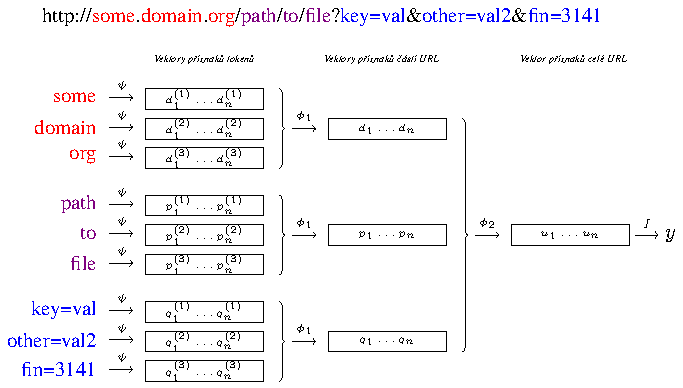
\includegraphics{images/model_MIL/model_MIL.pdf}
	\caption{Model adresy URL}\label{url_model_MIL}
\end{figure}

\section{Modifikace MIL pro tuto úlohu}\label{MIL-modification}
Každá adresa URL musí obsahovat doménu, avšak i adresy, kterým chybí cesta nebo dotaz (nebo dokonce cesta i dotaz), mohou být validními adresami URL ve smyslu \cite{berners-lee_uniform_1994}. Vzhledem k tomu, jak byl prostor \( \BPspace B_2 \) konstruován, je tedy zřejmé, že platí
\[ \left( \forall b \in \BPspace B_2 \right) \left( 1 \leq \left| b \right| \leq 3 \right) \]
Je ovšem možné chybějící části adresy URL reprezentovat jednou podčástí odpovídající prázdnému slovu abecedy \( \Sigma \) \footnote{Což nutně nemusí znamenat, že jsou reprezentovány nulovým vektorem příznaků.}. Díky tomuto rozšíření lze předchozí odhad velikosti tašek v prostoru \( \BPspace B_2 \) zesílit na
\[ \left( \forall b \in \BPspace B_2 \right) \left( \left| b \right| = 3 \right) \]

Protože doména, cesta a dotaz mají v adrese URL fundamentálně odlišný účel, nedává smysl, aby jim odpovídající vkládající funkce byly totožné. Rozšíření multi-instančního přístupu navržené v předchozím odstavci nám umožňuje nahradit funkci \( \phi_1 \) třemi různymi vkládajícími funkcemi \( \phi_D \), \( \phi_P \) a \( \phi_Q \), odpovídajícími doméně, cestě a dotazu respektive. Rovněž předpis pro vkládající funkci \( \phi_2 \) se díky konstantní velikosti tašek z prostoru \( \BPspace B_2 \) zjednoduší na
\[ \phi_2 : \BPspace X_2^3 \to \BPspace X_3 \]
Takto modifikovaná abstrakce je graficky znázorněna na obrázku \ref{url_model_modified_MIL}.

\begin{figure}[h]
	\centering
	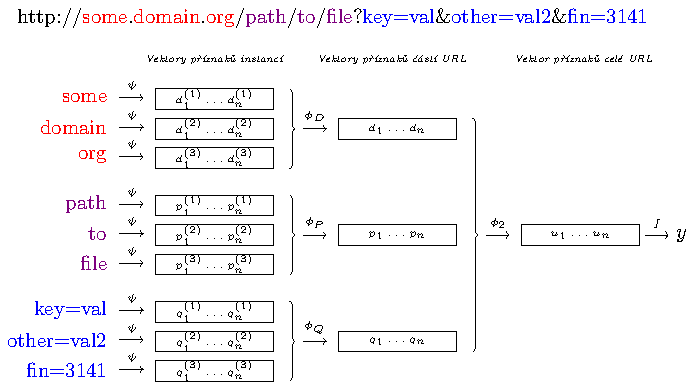
\includegraphics{images/model_modified_MIL/model_modified_MIL.pdf}
	\caption{Modifikovaný model adresy URL}\label{url_model_modified_MIL}
\end{figure}

\section{Metody hledání vkládající a klasifikační funkce}
Obecně lze v klasickém multi-instančním učení definovat vkládající funkci \( \phi \) jako
\begin{equation}\label{netpooling}
	\phi : \BPspace B \to \bar{\BPspace X} : b \mapsto g \left( \left\{ k \left( x \right) \middle| x \in b \right\} \right)
\end{equation}
kde 
\begin{align*}
	k &: \BPspace X \to \BPspace X \\
	g &: \bigcup_{m = 1}^{+ \infty} \BPspace X^m \to \bar{\BPspace X}
\end{align*}
Za \( g \) lze volit napříkald funkce minimum, maximum, aritmetický průměr. Funkce \( k \) je definována neuronovou sítí, která je trénována libovolným algoritmem pro učení s učítelem. Pokud jsou funkce \( k \) a \( f \) obě definovány neuronovou sítí, jsou tyto neuronové sítě trénovány společně.

V dalším textu budou předpokládány již konkrétní prostory, a to sice
\begin{align*}
	\BPspace X_1 &= \BPfield R^n \\
	\BPspace X_2 &= \BPfield R^n \\
	\BPspace X_3 &= \BPfield R^{3n} \\
	\BPspace Y &= \left\{ -1, +1 \right\}
\end{align*}
pro nějaké \( n \in \BPfield N \).

Přístup pomocí \eqref{netpooling} byl využit pro vkládající funkce první úrovně, tedy
\begin{align*}
	\phi_D &: \BPspace B_1 \to \BPfield R^n : b \mapsto g_D \left( \left\{ k_D \left( x \right) \middle| x \in b \right\} \right) \\
	\phi_P &: \BPspace B_1 \to \BPfield R^n : b \mapsto g_P \left( \left\{ k_P \left( x \right) \middle| x \in b \right\} \right) \\
	\phi_Q &: \BPspace B_1 \to \BPfield R^n : b \mapsto g_Q \left( \left\{ k_Q \left( x \right) \middle| x \in b \right\} \right)
\end{align*}
Za vkládající funkci druhé úrovně byla volena funkce konkatenace vektorů, tedy funkce \( \phi_2 : \left( \BPfield R^n \right)^3  \to \BPfield R^{3n} \) s funkčním předpisem
\begin{multline}
	\phi_2 \left( \left( x_1^{(1)}, \dots, x_n^{(1)} \right), \left( x_1^{(2)}, \dots, x_n^{(2)} \right), \left( x_1^{(3)}, \dots, x_n^{(3)} \right) \right) = \\
	= \left( x_1^{(1)}, \dots, x_n^{(1)}, x_1^{(2)}, \dots, x_n^{(2)}, x_1^{(3)}, \dots, x_n^{(3)} \right)
\end{multline}
Takto lze vkládající funkci \( \phi_2 \) volit pouze díky modifikaci navržené v kapitole \ref{MIL-modification}.

Klasifikační funkce \( f : \BPfield R^{3n} \to \left\{ -1, +1 \right\} \) je definovaná neuronovou síťí, která je trénovaná společně s neuronovými sítěmi definujícími funkce \( k_D \), \( k_P \) a \( k_Q \).


